\chapter{The Data Pipeline}
\label{ChapterIII}
\nocite{rgdal}
\section{Introduction}


The 13F-HR report is the cornerstone of this study, for it offers a very detailed peek into the stock holdings of all institutional investors with holdings above 100 million dollars USD in fair market value, as well as voluntary reports for firms with smaller holdings\footnote{Some institutional investors with holdings under 100 million USD are compulsory rather than voluntary in nature due to having exceeded the 100 million USD reporting threshold in the previous 4 quarters.}.  Understanding the data pipeline, that is to say how the data went from the SEC's Edgar server, wrangled into the databases, and then cleaned prior to use in statistical models is important in understanding the strengths and limitations of these models.  Otherwise it's garbage in, garbage out (GIGO) research.  

\section{The 13F-Holding Report}

There are countless news articles that use 13F-Holding Reports (13F-HR) data as a basis for ``whale watching", that is to say, poring over the 13F reports of successful investors such as, but not limited to Warren Buffet, and imitating their strategies and/or replicating their holdings on a smaller scale \citep{Whale_Watching_CNBC_12}.  While some may debate the wisdom of buying and selling stocks based on what experts were holding 45 days in the past\footnote{13F-HR reports are due to the SEC for public access no more than 45 days after the end of a quarter.  For example, reports for the period ending March 31st would be due no later than May 15th (or the next Monday if that date would fall on a Saturday or Sunday)}, other say that these reports allow smaller investors to gain insights based on the research departments of larger investors \citep{WhaleReport13}.  

The data for this thesis was collected from the SEC's Edgar database between 2015 and February \nth{18}, 2019.  The Edgar database provides 13F filings in two different formats.  The first of these formats is the ``.txt" format, which covers the period of March 31, 1999 to March 31, 2013. It should be noted that despite the existence of older filings on the Edgar server prior to March 31, 1999, these filings covering the time period of 1990 to 1998 only exist for a handful of filers each quarter and thus would provide an incomplete and biased sample.  This era of filings contain holding information in an unstructured format that are easily human readable, but unreliable when parsed by computers.  The second era of filing formats covers the periods of June \nth{30}, 2013 to December \nth{31}, 2018.  These filings are in the newer ``XBRL" file format which is a derivative of the popular ``XML" file structure.  This file format has the benefit of being easily machine readable.  Furthermore, all 13F-HR/A files represent amendments to previous filings were integrated in to the database. 

Due to the difficulties in parsing the older ``.txt" file formats, this mandated the creation of two different databases of institutional investors.  One piece of information that was easily extracted from the ``.txt" files was the business address of the investor.  This leads to the creation of a database containing what is essentially a ``phone book" information for all institutional investors that filed at least one quarterly report during the 20 year period covered by this research ($n = 242084$). The second database is derived from the ``XBRL" encoded files and contains a list of all positions reported by the filer to the SEC. Since some filers chose to disclose more information than required, and in the interest of maintaining a fair comparison across firms, only positions containing securities were kept in the database ($n=92539$).  

\label{Section:13F}

When plotting the duration of how long different filers (as defined by unique Central Index Key (CIK)) exist in the database, as seen in Figure \ref{fig:countoffilers}, one notices a pattern in the data where peeks can be found at $n+1$ quarters where $n$ is zero or an integer divisible by 4.  The most likely explanation for this reporting artifact is the requirement to report for the next four quarters after which they have fallen back under the 100 million dollar reporting threshold.   

\begin{figure}
	\centering
	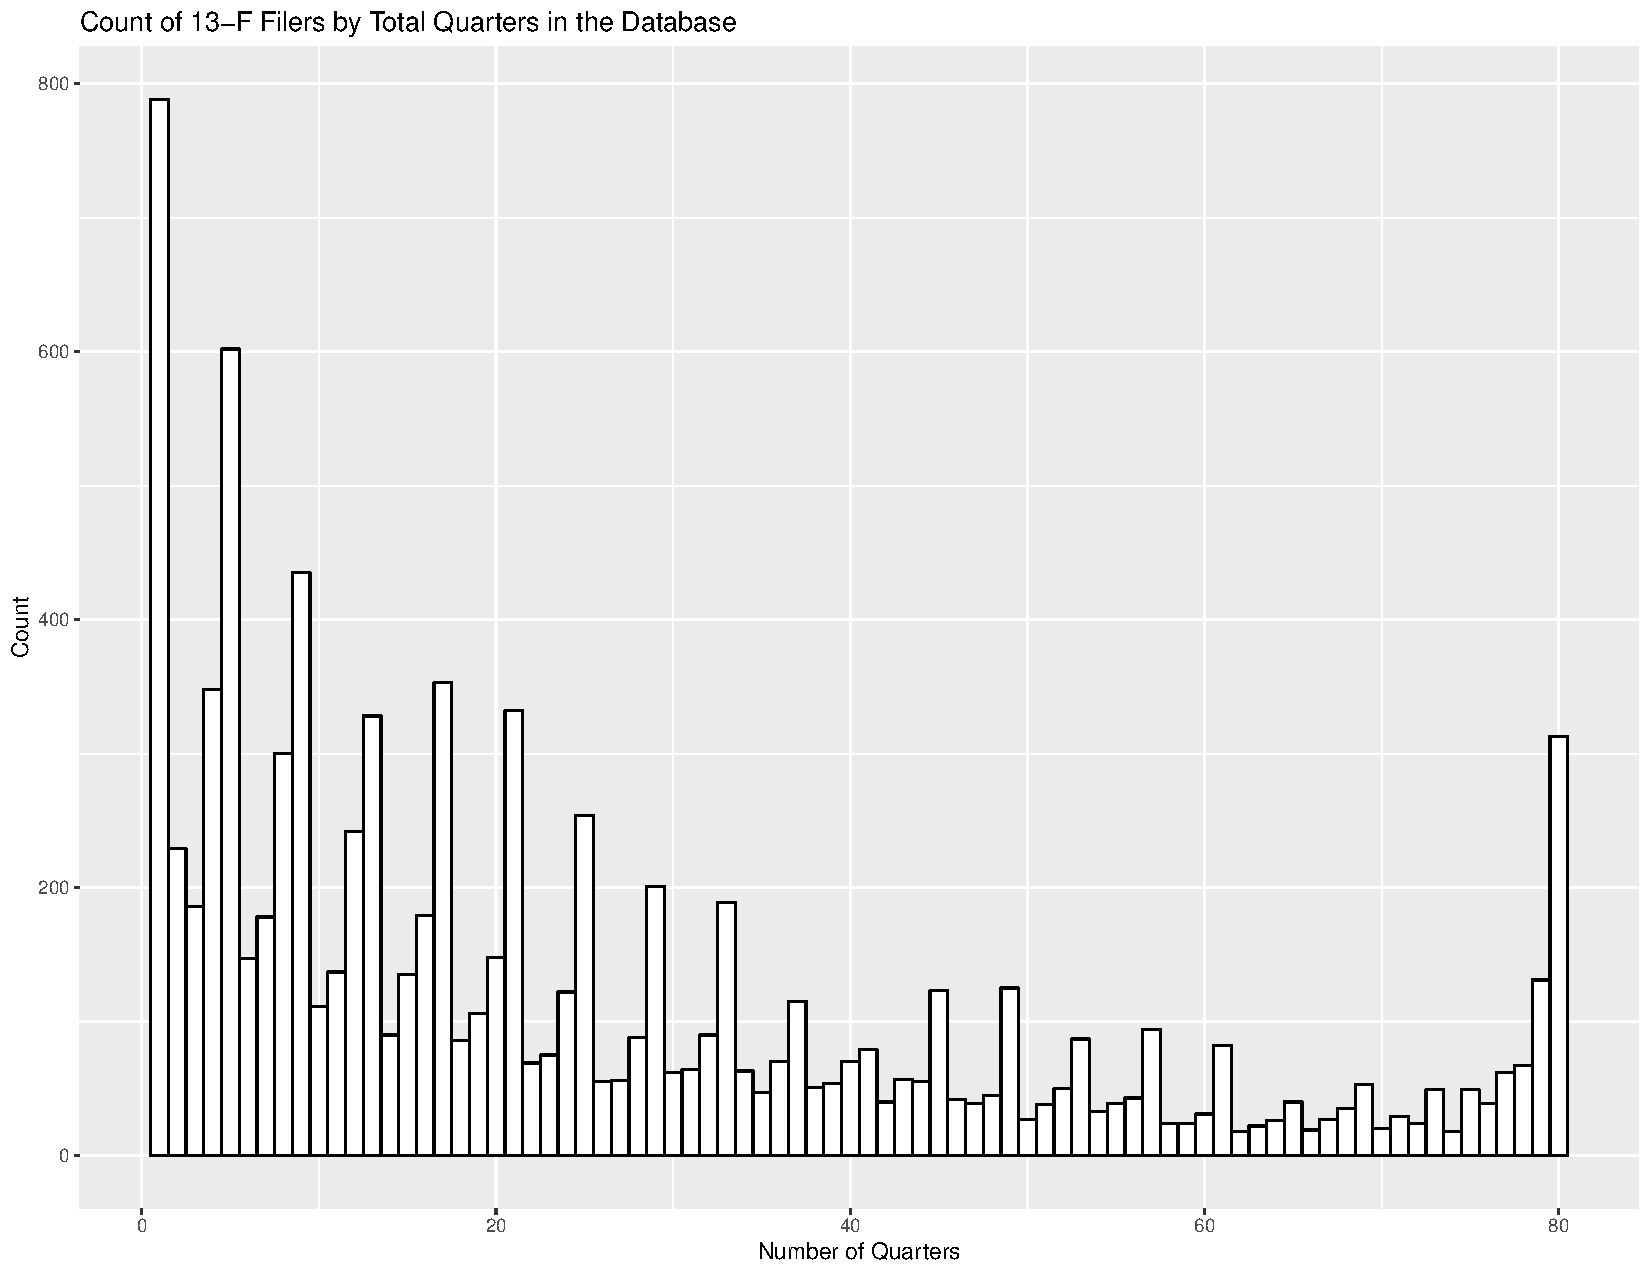
\includegraphics[width=1\linewidth]{Figures/ChapterIII/Count_of_Filers}
	\caption[Count of 13-F Filers by Quarter]{Count of 13-F filers by quarter in the EDGAR 13-F Database. One should note the regular pattern of $n+1$ quarters, where $n$ is zero or an integer divisible by 4.}
	\label{fig:countoffilers}
\end{figure}



\subsection{Investors by Country}


While these filings are filed under pain of perjury, there is no guarantee that these filings are a true and accurate reflection of the investor's books\footnote{For example, Bernie Madoff's fraudulent fund is still listed in the pre-2008 data}.  In fact, the SEC's EDGAR server warns users that they are not responsible for any damages caused by acting on incorrect information.  In line with this warning, it is obvious that some filings are incorrect.  In a few cases, one quarter's filings were orders of magnitude larger than all other filings reported by that filer.  For example, Firm 0000863748's filing for March \nth{31}, 2016 reported a total fund value of 5,632,710,967,874.14 USD.  This value is more than twice the value recorded for BlackRock family of funds, as well as being orders magnitude larger than the neighbouring filings.  While there is no absolute guarantee that all filings are accurate, the yearly totals were verified for anomalous values using the Rosner Test as found in the EnvStats R package \citep{EnvStats-book}. During the period of June 2013 to December 2018, there were 570 filings with anomalous top-line values flagged by the Rosner Test. However, not all abrupt changes in top-line valuation are due to erroneous filings.  One such example is BlackRock which underwent a change of reporting scheme for 2017 onwards, where it decided to consolidate more reports under one filing ( BlackRock Advisors, LLC, BlackRock Fund Advisors, BlackRock Investment Management, LLC, BlackRock Group Limited, BlackRock Institutional Trust Company, N.A. and BlackRock Japan Co., Ltd.), and thus went from reporting 70.6 billion USD to 1.8 trillion USD. For the suspect filings that could not otherwise be explained, these values were extracted from the database and replaced with a synthetic entry using a weighted average of the surrounding 4 quarters\footnote{The main weighting is a (0.2/0.3/suspect entry/0.3/0.2), however, June 2013 and first company filings are treated with a suspect entry/0.6/0.4 (opposite weights for last filing and December 2018), the filing for September 2013 and filers with suspect second entry is 0.4/suspect entry/0.4/0.2. (Inverse weights for September 2018 and December 2018)}. 

This is further complicated by the fact that the legal basis for 13F-HR disclosure mandates only the disclosure of securities and thus the conversion of an investment position to a non-reportable position has a warping effect on the top-line value for each fund. For example, if an investor were to convert a million dollar position in a company into a million dollars worth of real estate, the 13F-HR filing would show a drop of 1 million dollars in the subsequent filing, however the fund's true bottom line did not change.  Furthermore, research conducted by \cite{griffinhow2009} looked at the difference between institutional investors and mutual funds, and how they organize their respective short and long positions.  As a matter of law, mutual funds can't short stocks and thus are forced to make their profit off of their long positions.  By contrast, the hedge fund's more permissive regulatory regime allows for short-selling and thus allows for the set-up of using long positions for hedges, and short-selling as a profit-generator.  That being said, the researchers found that there is no statistical difference between the long position profitability between hedge funds and mutual funds.  As a consequence, the long positions as reported in the 13F-HR filings should still hold valuable insights in corporate command and control functions, especially since many firms have a waiting period before the power to vote on board of directors vest.  



\nomenclature{USD}{United States Dollar}

Interestingly, Bernard L. Madoff Investment Securities LLC (CIK number 00001386924) exists within the database from June 2006 to September 2008.  However, as was revealed in December 2008, Bernie Madoff was at the centre of a 50 billion USD Ponzi scheme \citep{Appelbaum2008} in which instead of investing his client's money, he would deposit investments into his personal bank account, as well as pay redemption from this account.   As Harry Markopolos detailed in his testimony to the House Financial Services Committee in the aftermath of the Bernie Madoff scheme's unravelling, use of 13F-HR should have uncovered the scheme years earlier, since what he reported on the disclosure form did not match what he was telling clients \citep{Marko09}.   Due to being a known fraud,  Bernard L. Madoff Investment Securities LLC (CIK number 00001386924) was censored from the database.  While it's unknown how many other fraudulent investment funds exist, there is no other choice than to believe that all the filings are done in good faith, and that the 570 anomalous filings were based on human error.  

\section{Tying Capital to Physical Space}

Financial Capital is inherently global while money often acts on the local scale \citep{clarkmoney2005}.  An apt metaphor according to Clark is that money will flow like mercury due to the following properties: 


\begin{quote}Characteristically, mercury tends to (1) run together at speed, (2) form in pools, (3) re-form in pools if disturbed, (4) follow the rivulets and channels of any surface however smooth it may appear to be, and (5) is poisonous in small and large doses if poorly managed. \citep[p105]{clarkmoney2005}
\end{quote}

These characteristics can make mapping global finance difficult. With the information available in the form 13F-HR, the best one can do to tie the command and control functions of the decision makers is to use the business address in which investors deal with the US regulatory system, and the Securities and Exchange Commission in particular. 


\section{The Time Period}
\begin{figure}[H]
	\centering
	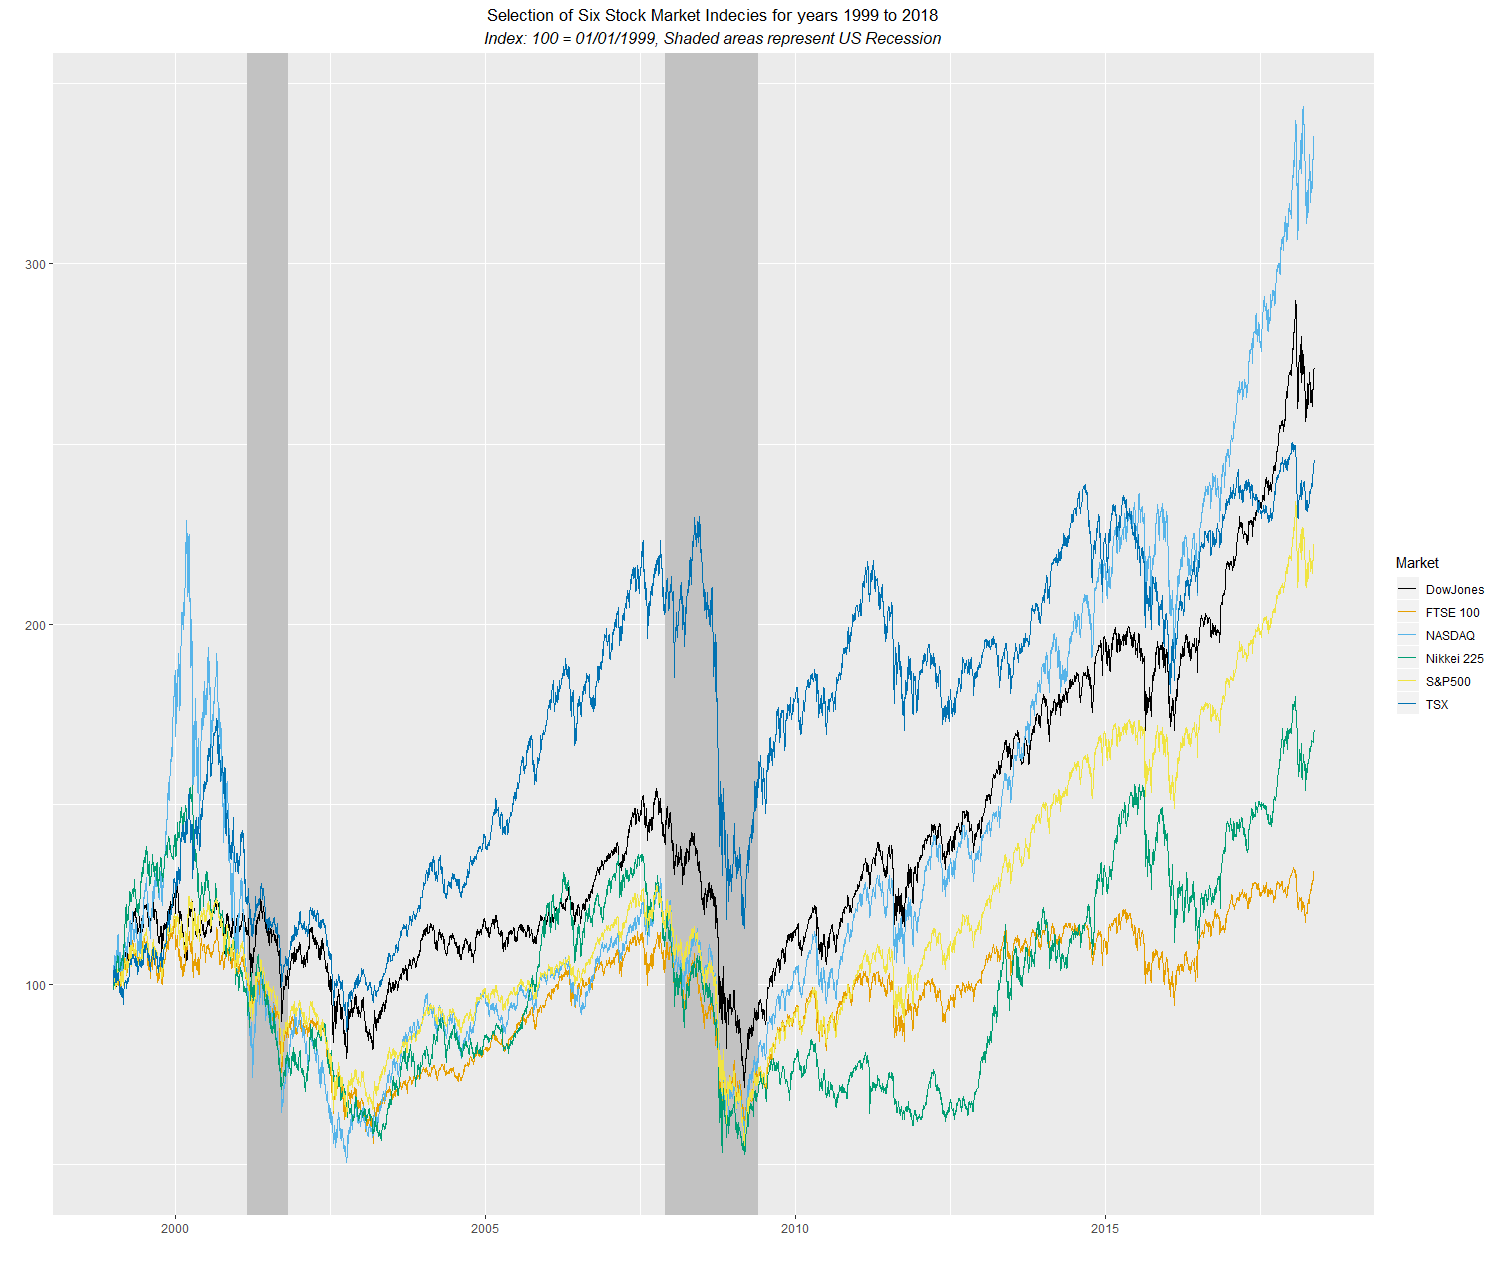
\includegraphics[width=1\textwidth]{Figures/ChapterII/Stock_Market}
	\caption[Stock Indices for 1999 to May 2018]{Collection of six stock indices for the years 1999 to 2018. The information was collected from Yahoo! Finance API on December 28, 2018.  Shaded Areas represent recessions as defined by the National Bureau of Economic Research's Business Cycle Dating Committee \url{https://www.nber.org/cycles/cyclesmain.html}.  The first recession dates from March 2001 to November 2001 and the second dates from December 2007 to June 2009. }
	\label{fig:stockmarket}
\end{figure}

Stock market indices provide a general guideline on the overall health of the stock market \citep{Lo21}.  From the investor's point of view, this is often used as a performance benchmark in which to evaluate their return \textit{vis-a-vis} their peers. Figure \ref{fig:stockmarket} shows a collection of six stock indices.  Three of these indices are used as bell-weathers of the US Stock-Market: The Dow Jones Industrial Average (DJIA/DOW)\footnote{The Dow Jones Industrial Average is an index of 30 blue chip US stocks covering the US economy except for transportation and utilities.  The mix of 30 stocks has changed over time to reflect changes in the economy \citep{DOW2020}.}, The Standard and Poors 500 (S\&P 500)\footnote{The S\&P 500 is an index of 500 large-cap stocks that tries to be representative of the US economy \citep{SNP2020}} and the National Association of Securities Dealers Automated Quotations Composite (NASDAQ Composite)\footnote{The NASDAQ is a broad-based index of over 3000 stocks listed on the NASDAQ stock exchange.  This index is heavily weighted towards the tech sector, and as such the ``irrational exuberance" of the DotCom era cast a large shadow over this index, taking 15 years to surpass to the record highs that were recorded during this era (NASDAQ, 2018)\nocite{NASDAQ2018}.}.   The three other indices give insights to the national stock markets of various important regions for this study.  The first is the UK's FTSE 100, Japan's Nikkei 225 and Canada's TSX.  

Examining the correlations over time of various stock index is beyond the scope of this thesis, one would be remiss to forget to draw attention to the correlated nature of the various stock indices.  That being said, being aware of the general nature of the stock market (Bear vs Bull market) gives context to whether growth in an investor's position can be partially explained by capital gains rather than attracting new clients and capital.  More specifically, the 20 year period of 1999 to 2018 is an era that can be characterised as having strong overall growth, punctuated by two rather large financial crises: the DotCom crash of 2000 and the Great Financial Crisis of 2008-2009.  As a consequence, this time period contains 2 powerful bull markets in which the market recovers powerfully from crash.  The first being the mid-aughts economic boom and the other the Obama recovery.



\nomenclature{NASDAQ}{National Association of Securities Dealers Automated Quotations Composite}
\nomenclature{S\&P 500}{The Standard and Poors 500 Index}
\nomenclature{DJIA}{Dow Jones Industrial Average}
\nomenclature{DOW}{Dow Jones Industrial Average}

While stock markets are somewhat useful in determining the scope and duration of a recession, \cite{Samuelson1966} oft-quoted quip of ``the
stock market has forecast nine of the last five recessions" has a certain amount of truth to it. This is why the significant stock market correction that took place in 2016 isn't shaded as a recession in figure \ref{fig:stockmarket}, since this did not have a significantly negative impact on the broader economy. This is why the National Bureau of Economic Research (NBER) does not have a fixed definition of what exactly constitutes a recession, going for an approach similar to Justice Potter Stuart's definition of obscenity - ``You know it when you see it" (Jacobellis v. Ohio, 378 U.S. 184. 1964). As such, the NBER's Business Cycle Dating Committee is charged at taking a holistic view of the economy when determining the length and breath of a recession such as changes in employment, housing starts, payroll numbers, manufacturing output and aggregate hours worked in the economy rather than fixate of certain metrics such as stock market contractions or changes in Gross Domestic Product \citep{NBERBCDC2020}.  




\section{Conclusion}


This section explores the data collection pipeline from the SEC's Edgar server to the decision to create two separate databases of 13F investors. As seen from the examples of inconceivable wealth declared in certain 13F-HR files due to various clerical errors, the data cleaning was an important factor in being able to trust the outputs of the models.  Furthermore, the inability to trust the semi-structured text format led to the creation of the "phone book" database and the more machine readable ``XBRL'' based database.  The first database covers the time period of 1999 to 2018 and contains what is essentially phone book information such as years active and locations. The more detailed ``XBRL'' based database covers the time period of June 2013 to December 2018.  This second database contains a detailed stock listing of their end of quarter holdings.  Both databases were then geocoded using Google Maps API.  Next, these databases were contextualized by exploring the time period in which they were active.  

In the following chapters, these databases will permit this paper to map the evolution of institutional investing in the United States for time periods they cover in order to examine if there are any significant changes in the hierarchies of cities from the time of \cite{greena1993} and \cite{gravesthe1998}.  Secondly, the more detailed database will allow for the examination of whether portfolio preferences play a role \textit{vis-a-vis} the locational choices of investors.  

